\subsection{Gestione di processo}

\subsubsection{Scopo}
Il processo di gestione, come stabilito nello standard ISO/IEC 12207:1995, contiene le attività e i compiti da utilizzare per la gestione dei rispettivi processi.\\
Il \respProg{} è responsabile per:
\begin{itemize}
\item il risultato della gestione;
\item la gestione del progetto stesso;
\item la gestione dei compiti del processo o dei processi ad esso applicabili.
\end{itemize}

\subsubsection{Descrizione}
Le attività di gestione di processo sono:
\begin{itemize}
\item inizio e definizione dello scopo;
\item istanziazione dei processi;
\item pianificazione e stima di costi, risorse e tempi;
\item assegnazione dei ruoli e dei compiti;
\item esecuzione e controllo;
\item revisione periodica delle attività.
\end{itemize}

\subsubsection{Coordinamento}

\myparagraph{Scopo} In questa sezione vengono esposte le norme di coordinamento relative alla comunicazione interna tra i membri del gruppo, e esterna con proponenti e committenti, con una panoramica degli strumenti che verranno utilizzati.

\myparagraph{Aspettative} Gli obiettivi sono di:
\begin{itemize}
	\item{facilitare la comunicazione tra i membri del gruppo mediante l'assegnazione di ruoli e obiettivi da raggiungere;}
	\item{monitorare il team con l'obiettivo di avere sotto controllo l'avanzamento del progetto.}
\end{itemize}

\subsubsection{Descrizione}
In questo modulo, chiamato \textbf{Back-end\ped{G}}, viene gestita la logica interna del sito \nameproject. In particolare viene amministrato l'accesso al lato \textbf{business} dell'applicativo, e la parte relativa alla persistenza dei dati salvati all'interno dei servizi offerti da Amazon AWS\ped{G}. L'architettura generale del modulo è basata sui microservizi offerti dalle chiamate API, i quali hanno una base in comune sviluppata a \textbf{layer}, dove i tre layer principali sono:
\begin{itemize}
	\item \textbf{Handler\ped{G} delle API\ped{G}}: gestori delle richieste suddivise per dominio;
	\item \textbf{Model}: gestione logica dei modelli delle entità rappresentate (prodotto, utente...);
	\item \textbf{Services}: gestione dei servizi Amazon AWS\ped{G} e complementari.
\end{itemize} Il modulo \textbf{Front-end\ped{G}} interagisce con il modulo \textbf{Back-end\ped{G}} attraverso delle chiamate API\ped{G} esposte del servizio Amazon API Gateway. Tali API\ped{G} sono divise per dominio relativo all'oggetto con cui si vuole interagire e alla sua funzionalità (es. inserimento di un nuovo prodotto). L'handler\ped{G} gestisce la richiesta in base alla propria funzionalità e smista la relativa richiesta, dopo un opportuno controllo, sul \textbf{layer dei servizi} (dove necessario). I servizi offerti comprendono l'interfacciamento con DynamoDB, Stripe, S3, Nodemailer, Cognito. Inoltre, sempre dove necessario, l'handler\ped{G} della richiesta può interfacciarsi con il \textbf{layer dei modelli} degli oggetti (prodotto, utente ecc..) i quali forniranno supporto per la gestione logica di tali elementi.

\vspace{1cm}

\begin{figure}[H]
\centering
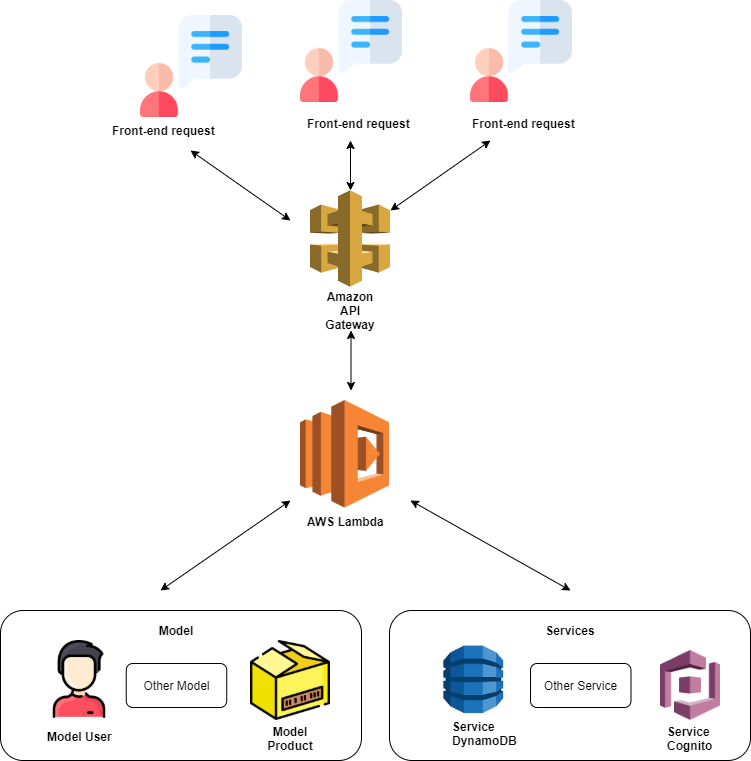
\includegraphics[scale=0.40]{res/Architettura/Backend/img/layerBack-end.png}\\
\caption{Layer del modulo Back-end\ped{G}}
\end{figure}

\subsubsection{Procedure}
\myparagraph{Gestione delle comunicazioni}
Le comunicazioni possono essere interne, cioè coinvolgono solo i partecipanti del team, oppure esterne, cioè includono anche soggetti esterni come proponente e committente.
\begin{itemize}
	\item \textbf{Comunicazioni interne}: per le comunicazioni tra i membri del gruppo è stato adottato Discord\ped{G}, un'applicazione VoIP multi piattaforma. Su Discord\ped{G} si possono integrare bot\ped{G}, creare canali tematici per rendere più efficiente lo scambio e il reperimento delle informazioni. \\
	All'interno di Discord\ped{G}, sono stati predisposti i seguenti canali tematici:
	\begin{itemize}
	\item \textbf{general}: per le comunicazioni di carattere generale;
	\item \textbf{github-updates}: canale riservato nel quale un bot\ped{G} automatico invia notifiche con i risultati delle \textit{GitHub Actions}\ped{G} (§3.4.5.2) ed ogni volta che un membro del team effettua una \textit{push}, apre/commenta/chiude una \textit{issue}, effettua un \textit{merge} su GitHub\ped{G};
	\item \textbf{resources}: per la condivisione di link utili;
	\item \textbf{date-incontri}: per decidere, in base alle disponibilità individuali, quando fissare riunioni;
	\item \textbf{template}: canale dedicato alla creazione del template\ped{G} di tutti i documenti e alla sua manutenzione nel tempo;
	\item un canale per ciascun documento in modo da avere una migliore organizzazione del contenuto di essi. 
	\end{itemize}
	\item \textbf{Comunicazioni esterne}: le comunicazioni con soggetti esterni al team sono di competenza del \respProg . I soggetti esterni con il quale intrattenere rapporti utili sono:
	\begin{itemize}
		\item i Committenti \textbf{\VT} e \textbf{\CR}, con cui si userà l'indirizzo \url{omicronswe@gmail.com};
		\item il Proponente \textbf{\Proponente}, con cui si è deciso di utilizzare un canale Slack\ped{G} per la chat testuale e il servizio Google Meet\ped{G} per le videochiamate.
	\end{itemize}
\end{itemize}

\myparagraph{Gestione degli incontri}
Gli incontri possono essere esterni o interni, sulla base della partecipazione di soggetti esterni al team o no. Per entrambe le tipologie di incontro, il \respProg{} nomina un segretario che avrà il compito di redigere il verbale dell'incontro.
\begin{itemize}
\item \textbf{Incontri interni}: il \respProg{} ha il compito di organizzare gli incontri interni utilizzando il canale Discord\ped{G} dedicato, dove ci si accorda con i membri del gruppo sul miglior timeslot;
\item \textbf{Incontri esterni}: il \respProg{} ha il compito di comunicare ed organizzare gli incontri esterni con il proponente o il committente, decidendo una data in comune accordo con le parti.
\end{itemize}

\myparagraph{Gestione degli strumenti di coordinamento}
Per suddividere il carico di lavoro in task\ped{G} che saranno poi divisi tra tutti i componenti, viene usata la funzionalità \textit{Projects}\ped{G} di GitHub\ped{G}. La procedura per l'assegnazione di un task\ped{G} segue il seguente schema:
\begin{itemize}
\item creazione di una nuova issue\ped{G} con un titolo significativo e una breve descrizione se necessaria;
\item indicare la/e persona/e a cui è stato assegnato tale compito;
\item selezionare il projects\ped{G} a cui fa riferimento il compito;
\item indicare una milestone\ped{G}.
\end{itemize}
Ogni compito passa attraverso i seguenti stati:
\begin{itemize}
\item \textbf{To do}, da fare;
\item \textbf{In progress}, in lavorazione;
\item \textbf{Done}, completato.
\end{itemize}
Una volta che i compiti sono stati eseguiti, viene aperta una pull request\ped{G} che verrà chiusa solo dopo la fase di verifica e approvazione.

\myparagraph{Gestione dei rischi}
Un altro compito del \respProg{} è quello di rilevare i rischi e renderli noti tramite il \PdP. \\
Per la gestione dei rischi, la procedura da seguire è la seguente:
\begin{itemize}
\item individuare nuovi problemi e monitorare i rischi già previsti;
\item aggiungere i nuovi rischi nel \PdP;
\item ridefinire, se necessario, le strategie di progetto.
\end{itemize}

\myparagraph{Strumenti}
Durante lo svolgimento dell'intero progetto il gruppo utilizzerà questi strumenti:
\begin{itemize}
	\item \textbf{Telegram}\ped{G}: applicazione di messaggistica utilizzata per la gestione del gruppo nella fase iniziale;
	\item \textbf{Discord}\ped{G}: strumento per la gestione del gruppo e per le relative comunicazioni e video chiamate interne del team;
	\item \textbf{Slack}\ped{G}: strumento utilizzato per le comunicazioni con il proponente;
	\item \textbf{Google Meet}\ped{G}: strumento utilizzato per le video chiamate con il proponente;
	\item \textbf{Google Calendar}\ped{G}: strumento utilizzato dai membri di \Omicron{} per avere sotto controllo gli impegni di ogni membro e permettere una più semplice organizzazione degli incontri.
\end{itemize}

\section{Pianificazione}
